\documentclass[10pt,a4paper]{article}
\usepackage[utf8x]{inputenc}
\usepackage{ucs}
\usepackage{amsmath}
\usepackage{amsfonts}
\usepackage{amssymb}
\usepackage{graphicx}
\usepackage{threeparttable}
\usepackage{colortbl}
\usepackage{slashbox}
\usepackage{verbatim} % For multi-line comments
% For pseudo
\usepackage{algorithmic}
\usepackage{algorithm}
\numberwithin{algorithm}{section}  % <--- chapter, section etc. depending on what is required



\author{Quoc Anh Le}
\begin{document}
\section{Automatic BET Question Answering}
%- Automatic BET: explain the processing and how it works
%
%- Works on transcript (tested with both human and ASR)
%
%- Describe the stages, the pre-processing, also here the "training"

The system proceeds in three stages. In the first stage, known as a pre-processing, two questions and meeting transcript are normalized and reorganized in order to enhance the performance of algorithm. The second stage identifies a snippet of the meeting transcript or a passage which is most likely to contain the answer (i.e the facts that discriminate between the true and the false statement). The third stage compares the two candidate statements based on the identified paragraph(s), and returns the true one. 

Figure \ref{stages_of_system} gives an overview of the system. 

\begin{figure}[htbp]
\label{stages_of_system}

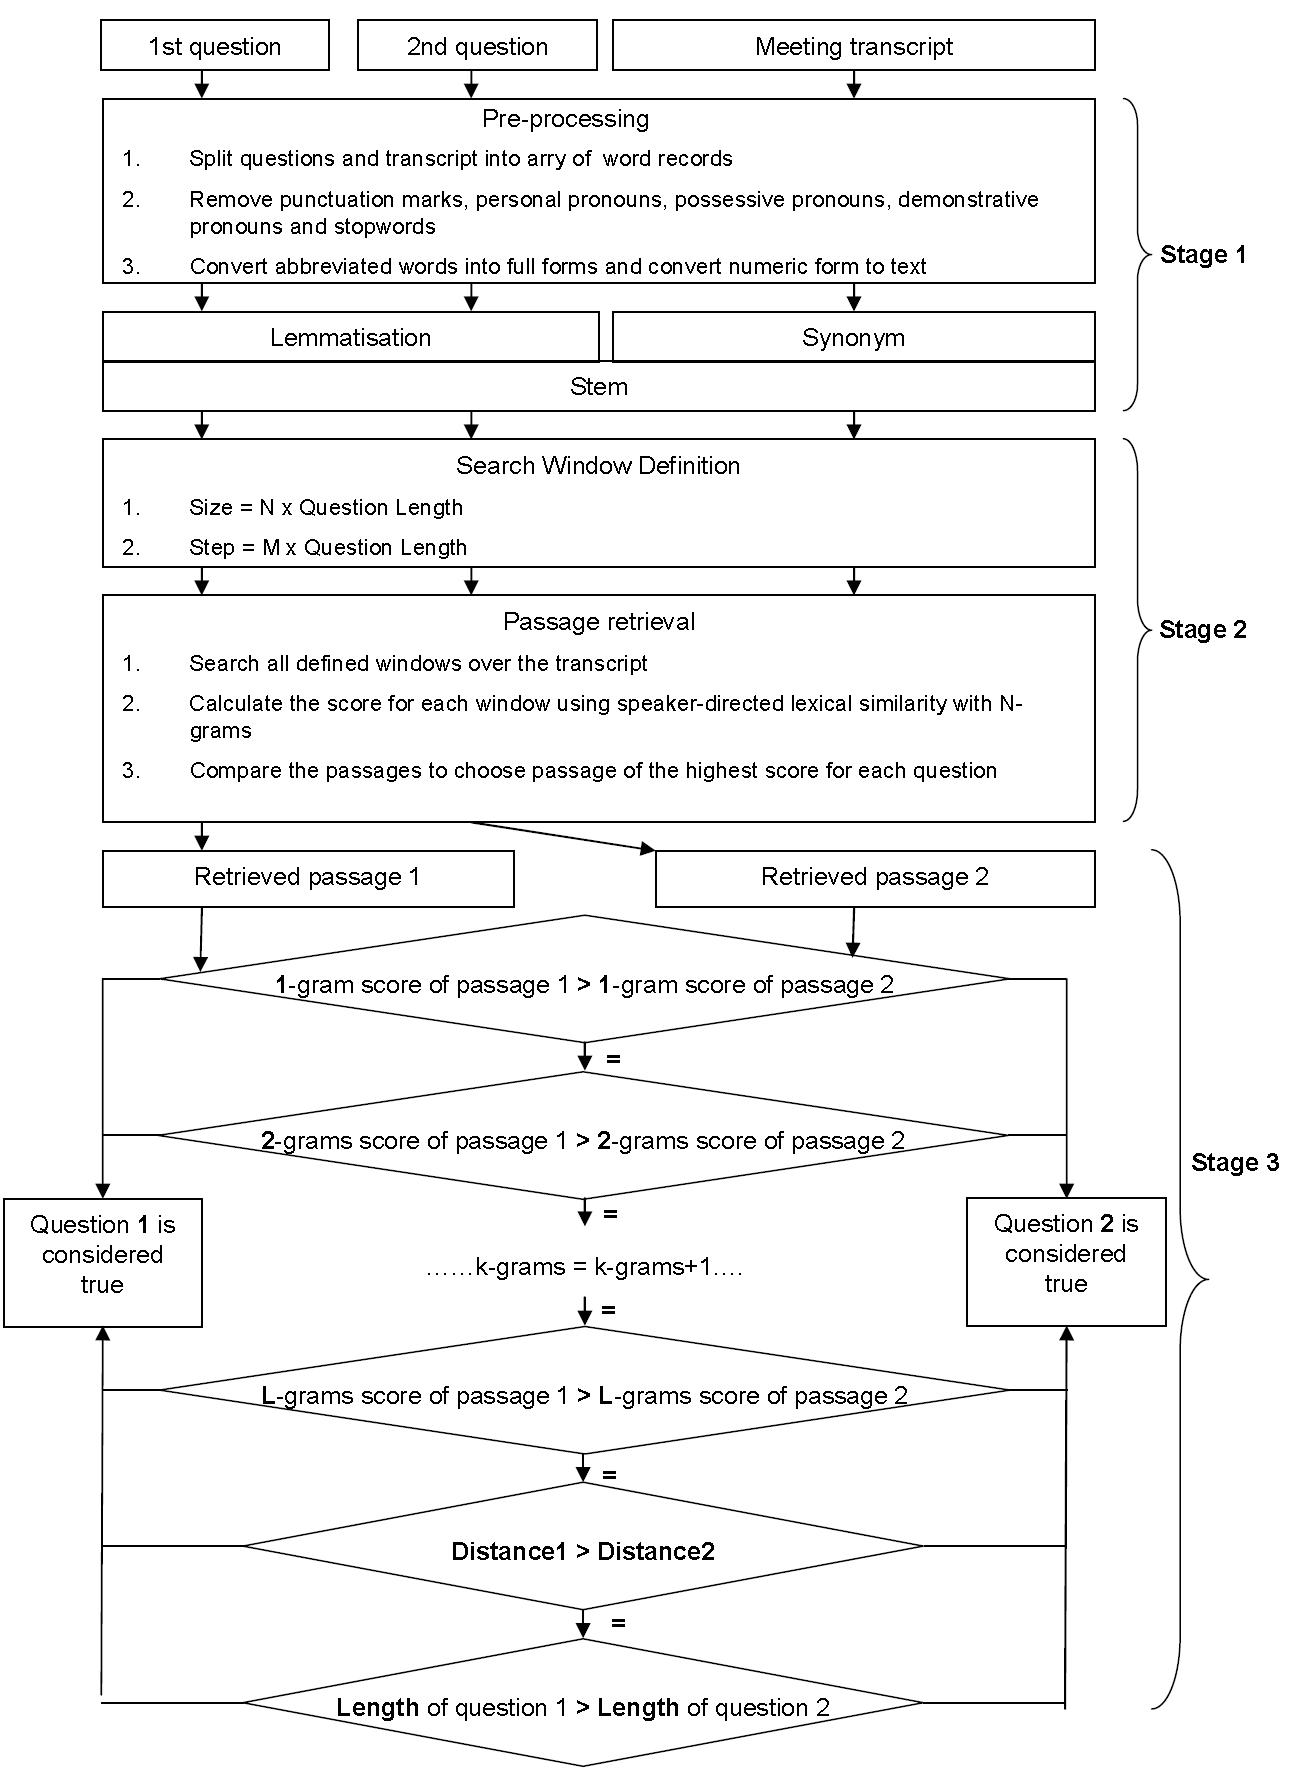
\includegraphics[scale = 0.4]{Stages_of_system.jpg}
\caption{Overview of the system}
\end{figure}


\subsection{Pre-processing}
There are two main tasks for this section. Firstly, text data are transformed into a unique text so that questions and transcript are treated in the same way. Secondly, meaning of word data is extended by lemma, stem and synonyms in order to enhance the performance of proposed algorithm.

The text processing are done by five operations as follows:

\begin{enumerate}
\item {Removing characters as punctuation marks: comma, dot, quotation mark, semicolon or exclamation, ect...  because these characters do not have any effect on the proposed algorithm based on lexical similarity. } 

\item {Removing stop-words such as "the", "to" or "for" that generally add little or no information regarding the subject matter of text \cite{mckechnie2001cap}. This helps to reduce cost of computing as well as to take precaution that they muddle the signal from the more content words \cite{hirschman1999drr}}

\item {For the reason that the questions are indirect-speech statements meanwhile the the meeting transcript is a direct-speech report, words that may be changed by a transformation from direct speech to indirect speech should be avoided from counting matched word between a question and a passage of the transcript. They are personal pronouns (I, me, myself, you, \ldots), possessive pronouns (my, your, \ldots), demonstrative pronouns (this, that, \ldots).}



\item {Converting numeric forms to text forms: 34 \ensuremath{\rightarrow} thirty four, 2nd \ensuremath{\rightarrow} second, etc \ldots so that they are written in the same way, this prevents an unnoticed matching while the algorithm executes. }

\item {Converting abbreviated words into full forms: We've \ensuremath{\rightarrow} We have, I'll \ensuremath{\rightarrow} I will, etc \ldots. This operation also helps the system treat the text in the same way.}
\end{enumerate}

The proposed algorithm uses lexical similarity to find a relevant passage that contains information of answer, thus a lexical extension should be added so that the system have more than one possibility of a matching between two words, for instance, production and product are matched each other because they have the same stem. 

Three lexical extensions are added to each word are lemma, stem and synonyms: i) Lemma is the canonical form of a word; ii) Stem is used to remove inflectional affixes; ii) synonyms which have same meaning with the original word. 


A question word are extended by adding its lemma, meanwhile the transcript words are extended by adding a set of synonyms. Stem is applied as the last operation on each word. This may increase the signal from contentful words, for instance for a question word as verb "modified" and a transcript word as noun "modification". There are not any matching between these words, even after doing a lemmatisation and a synonym.  In detail, "modified" becomes "modify" by a lemmatisation and "modification" has five synonyms "alteration adjustment qualifying limiting change" returned by WordNet \cite{pasca2001irw}. But after stemming by Snowball \cite{porter2001ss}, two words have a same form as "modifi" so that they are matched.

In practice, for each word, the programme runs a Stemming API of Porter, called Snowball \cite{porter2001ss} to obtain a stem and using WordNet API \cite{pasca2001irw} to obtain a lemma and a set of synonyms.

A set of synonyms is reduced to be more meaning with original word by using part of speech (PoS) tool QTAG API \cite{manson1997qpp} to remove synonyms that do not have the same PoS with the original word.  

Each word will be treated as a record of many fields. For a question word, it has three fields: original word, lemma of the word, stem of the lemma. They are described as the table \ref{Word splitting and lexical extensions for questions}. For a transcript word, it has five fields: original word, stem of word, name of speaker who spoke this word, set of synonyms and part of speech. They are described as the table \ref{word_splitting_transcript} The name of speakers in the transcript table is also stemmed in order to compare with a question word which may be a speaker name. This field is very important to measuring similarity between a question and a passage in the passage retrieval of the algorithm.

The fields \textit{synonyms} and \textit{lemma} are structured as a set of words. For example, lemma of "better" has two words "good" and "well", synonyms of "better" are "break improve amend ameliorate meliorate".

All steps above are processed in a procedure separated from execution of the main algorithm that includes passage retrieval and disambiguation. Questions and transcript returned from this stage are stored on hard disk so that the programme can load them into RAM before running the main algorithm. This saves us much time to experiment on different configurations of the algorithm.

For instance, for the pair of questions "Mirek had not received the agenda for the meeting" and "Andrei had not received the agenda for the meeting". After removing stop-words, they become "Mirek had not received agenda meeting" and "Andrei had not received agenda meeting". Their lexical extensions are presented as following table:

%\footnotesize

\begin{table}[htbp]
\scriptsize
\caption{Word splitting and lexical extensions for questions}
\begin{tabular}{|c|l|l|l|l|c|l|l|l|}
\hline
\multicolumn{ 4}{|c|}{\textbf{Question 1}} &  & \multicolumn{ 4}{c|}{\textbf{Question 2}} \\ \hline
\textbf{Position} & \multicolumn{1}{c|}{\textbf{Word}} & \multicolumn{1}{c|}{\textbf{Lemma}} & \multicolumn{1}{c|}{\textbf{Stem}} &  & \textbf{Position} & \multicolumn{1}{c|}{\textbf{Word}} & \multicolumn{1}{c|}{\textbf{Lemma}} & \multicolumn{1}{c|}{\textbf{Stem}} \\ \hline
1 & Mirek & Mirek & Mirek &  & 1 & Andrei & Andrei & Andrei \\ \hline
2 & had & have & have &  & 2 & had & have & have \\ \hline
3 & not & not & not &  & 3 & not & not & not \\ \hline
4 & received & receive & receiv &  & 4 & received & receive & receiv \\ \hline
5 & agenda & agenda & agenda &  & 5 & agenda & agenda & agenda \\ \hline
6 & meeting & meet & meet &  & 6 & meeting & meet & meet \\ \hline
\end{tabular}
\label{Word splitting and lexical extensions for questions}
\end{table}

\normalsize



For instance, for a snippet of transcript as below:
\scriptsize
\begin{verbatim}
.....
 Andrei Hi everyone. 
 Denis  So I don't know if you all received the the a- agenda for this meeting.
 Denis 	Do you - no?
 Mirek 	No, I haven't.
....
\end{verbatim}
\normalsize

After the processing, it becomes:
\scriptsize
\begin{verbatim}
.....
denis   9 not 10 know 11 if 12 you 13 all 14 received 18 agenda 21 meeting
denis   24 no 
mirek   25 No 27 have 28 not
....
\end{verbatim}
\normalsize

and it is transformed into the following table:

\begin{center}
\begin{threeparttable}
\scriptsize
\caption{Word splitting and lexical extensions for transcript}
\label{word_splitting_transcript}
\begin{tabular}{|c|l|l|c|l|l|}
%\hline \multicolumn{6}{|c|}{Word splitting} \\
\hline  \bf{Position} & \bf{Word} & \bf{Stem} & \bf{Speaker} & \bf{Synonyms} &\bf{PoS} \\
\hline \ldots & \ldots & & & &\\
\hline 9 & not & not & deni & non & XNOT\\
\hline 10 & know & know & deni & cogniz experi live acknowledg recogn \ldots & VB\\
\hline 11 & if & if & deni & & CS\\
\hline 13 & all & all & deni & entir complet total altogeth whole  \ldots & PDT\\
\hline 14 & received & receiv & deni & have get find obtain \ldots &VBD\\
\hline 18 & agenda & agenda & deni & docket schedul agendum \ldots & NN\\
\hline 21 & meeting & meet & deni & fill match ensembl contact \ldots & NN\\
\hline 24 & no & no & deni & nobelium & DT\\
\hline 25 & no & no & mirek & nobelium & DT\\
\hline 27 & have &have &mirek &  receiv get own possess \ldots &HV\\
\hline 28 & not &not &mirek & non&XNOT\\
\hline \ldots & \ldots & & & &\\
\hline 
\end{tabular}
\end{threeparttable}
\end{center}


\normalsize
\subsection{Passage Retrieval}

% definition of a passage must be mentioned in the state-of-the-art
A passage can simply be defined as a sequence of words regardless sentences or paragraphs. Some text-based information retrieval systems define a passage as a fixed-length block of words. \cite{goharian2008dsp}

The goal of this stage is to retrieval a passage which is the most likely to contain information about the answer. Thus, this stage plays the most important role to the system because its performance decides accuracy of the system. Furthermore, it also gives a confidence of the performance that the final answer returned by the system may be true but the retrieved passage is not correct at all.

In order to find the relevant passage, the system have to compare all possible passages in the transcript. Information compared is passage score, which is a numeric value used to measure the similarity between a passage and a question.  The comparison is done by moving a search window from one place to another. If we assume that the transcript is a cloth stretched to be ironed, then the search window is iron. In the same way of using iron, the search window passes over all possible passages in the transcript. These passages have the same size with the window. At each time, the score of a passage that the window arrives is calculated and then returned in order to compare with passages that window arrived in the past so that passage of highest score are retrieved. 

There are many ways to calculate the score of a passage with respect to the question. However, according to the experimental results of Stefanie \cite{tellex2003qep} on different algorithms of passage retrieval, the performance of each algorithm is different from each other that depends on input data. That means each method is suitable for only some particular cases. Moreover, existing passage retrieval algorithms use input documents returned by a document retrieval system that returns unknown-typed documents such as a forum website, a commercial website or an online newspaper,... Additionally, these approaches have to analyse the type of questions such as "How" or "When" before doing a passage retrieval  \cite{TREC8, TREC2001, hirschman2002nlq, tellex2003qep}. This effects to final results of passage retrieval algorithm because each step causes an erroneous proportion. In our case, the type of document and the type of questions are defined clearly. That is why we do not apply any existing complex algorithms but develop our algorithm from a basic algorithm presented by Light et al. \cite{light2002aec} by adding some improvements to this algorithm. This is the simplest method to calculate a passage score that counts the number of common word between the passage and the question as passage score. Based on this method, we added four different matchings between a question word and a passage word. They are n-gram matching, lemma matching, stem matching, synonym matching and speaker matching. Lexical extensions such as lemmatisation, stem and synonyms are presented in the previous section. Applying n-gram matching and speaker matching are explained in detail as below.

As a convention, the term "matched word" is used to indicate that a question word which is found in a passage. In other words, they are words that the passage has in common with the question.


Basically, the score of a passage is based on the number of matched words as described by Light et al. However, there are three score levels assigned to matched words. A matched word as name of speakers have the highest score. That means passage score increases if the name of a speaker is containned in both question and question. A matched word as a synonym of original word have the lowest score. Other matched words as lemmatisation of original word have score assigned in the two ways that depend on if speaker matching exists or not.

As described in the table \ref{word_splitting_transcript}, each transcript word is corresponding to one speaker name. This is a characteristic of meeting transcript that we can benefit. If a matched word is spoken by a speaker whose name is addressed in the question, score assigned to this word must be add a bonus. 

In our experiment system, as described in the pseudo code \ref{alg: Passage Score}, different values of score assigned to a matched word as follows: 1) 4.0 if this word is a speaker name, 2) 0.5 if it is a synonym, 3) 2.5 if this word is spoken by a speaker whose name is containned in the question, 4) 1.0 for other cases.

All words are transformed into lower-case forms so that nouns, pronouns, verbs,... are treated in the same way. 

As mentioned above, a search window is used to search and calculate all possible passages on the transcript. Size of the search window is defined as a multiple of question length. Meanwhile, distance between two consecutive windows is known as window step and defined also as a multiple of question length. For instance, window size = 5 x question size and window step = 2 x question size. Thus, parameters of search window are dynamic that depend on input question. This method seems to be suitable to retrieve relevant passage using lexical similarity algorithm because when the length of the question increases, the information that question demands is larger. Thus, it is necessary to enlarge the size of search window.

At the first time, the passage retrieval algorithm return a list of highest-score passages but we know that only one relevant passage is corresponding to each BET question. To solve this problem, 2-gram matching, 3-gram matching,..., n-gram matching is applied to reduce the number of passages in the returned list, in which n is number of question words. N-gram score is calculated as follow: Instead of working on common words between question and passage, the programme will work on common sub-strings of n words between them. If two passages have same 1-gram score, their 2-gram score are compared with each other to return higher-score passage. If they have the same 2-gram score, their 3-gram score are compared with each other. And continuing in the same way until their score is different or their n-gram score are compared with each other that n is number of question words. The higher-score passage is returned as more relevant passage. If they still have the same n-gram score, it is not important which one is returned.


Implementation of calculating passage score is described by pseudo codes \ref{alg: Passage Score} with comments in detail. There are some remarks for this as follows:

- A passage is defined as a data record that has 5 properties: 1) Passage score shows the similarity between this passage with the current question; 2) Position of the passage in the transcript; 3) Size of passage; 4) Set of positions of matched words in the transcript; 5) Distance among matched words. This distance is calculated as sum of absolute distance of any matched word. This task is done at the end of the passage retrieval to prepare for the disambiguation stage of the algorithm.


- The priority order is given to "name matching", then "stem matching" and lastly "synonyms matching" in order to bring the highest score for the current passage.

- The values (4.0, 2.5, 1.0, 0.5) are determined by personal experiences. They are scores assigned to matched word in according as its context defined above.

- The frequency of one matched word is not used to increase the score. However, in the case of "multiple matching", if one word is repeated more than one time in both question and transcript, the score will be calculated as the minimum number of appearances of this word between the question and the transcript. 



\newpage


% Chia lam 2 cot, cot ben phai dung de viet comments
\begin{algorithm}   {ht!}                   % enter the algorithm environment
\caption{Passage Retrieval}          % give the algorithm a caption
\label{algo: Passage Retrieval}                           % and a label for \ref{} commands later in the document
\begin{algorithmic}       [1]             % enter the algorithmic environment
\small
\REQUIRE Question \COMMENT {Array of question word records as described in the table \ref{Word splitting and lexical extensions for questions}}
\REQUIRE Transcript \COMMENT{Array of transcript word records as described in the table \ref{word_splitting_transcript}}
\REQUIRE WindowSize \COMMENT {Size of search window (word unit)}
\REQUIRE WindowStep \COMMENT{Distance between two consecutive windows (word unit)}

\STATE $Passage \gets Empty$ \COMMENT{Initiate a new passage as current passage(The passage class is defined above)}
\STATE $BestPassage \gets Empty$ \COMMENT{Initiate a new passage as the best retrived passage at one moment}

\STATE $Position \gets 0$ \COMMENT{Initialized position of the search window}
\WHILE[Search for all passages to choose the best passage]{$Position \ensuremath{<} Transcript.length-WindowSize$} 
	\STATE $Passage.position \gets Position$ \COMMENT{Position of current passage}
	\STATE $Passage.size \gets WindowSize$   \COMMENT{Size of current passage}
	\STATE $Passage.WordList \gets Transcrip[Postion \div Position+WindowSize]$ \COMMENT{List of passage word records is extracted from the transcript[Position,Position+1,..,Position+Size of window]}
	\STATE $Ngrams \gets 1$ \COMMENT{Firstly, passage score is calculated using unigram matching}	
	\STATE $Passage.MatchedList \gets getMatchedList(Passage,Question,Ngrams)$ \COMMENT{Save matched words}
	\STATE $Passage.score \gets getPassageScore(Passage,Question,Ngrams)$ \COMMENT{Save score}
	
	\IF[The current passage is better]{$BestPassage.score \ensuremath{<} Passage.score$} 
		\STATE $BestPassage \gets Passage$ \COMMENT{remember it as the best passage}
	\ELSIF[If they have the same score]{$BestPassage.score \equiv Passage.score$} 
		\WHILE[Recalculate their score using bigrams, trigrams,.. until their score is different from each others or Ngrams is over the length of question ]{$BestPassage.score \equiv Passage.score \wedge Ngrams \leqslant Question.length $}
			\STATE $Ngram \gets Ngrams+1$ \COMMENT{Increase Ngrams by 1}
			\STATE $BestPassage.score \gets getPassageScore(BestPassage,Question,Ngrams)$ \COMMENT{Recalculation with new Ngrams}
			\STATE $BestPassage.score \gets getPassageScore(BestPassage,Question,Ngrams)$ \COMMENT{Recalculation with new Ngrams}
		\ENDWHILE
		\IF[Finally, if current passage have better score, remember the current passage as the best passage until now]{$BestPassage.score \ensuremath{<} Passage.score$} 
			\STATE $BestPassage \gets Passage$
		\ENDIF
	\ENDIF
	

	
	\STATE $Position \gets Position+WindowStep$ \COMMENT{Move the search window forward}
	
\ENDWHILE


%Distance
\STATE $Passage.distance \gets 0$
\FOR{$i=0$ to $Passage.WordList.Length-1$}
	\FOR{$j=i+1$ to $Passage.WordList.Length$}
		\STATE $Passage.distance  \gets Passage.distance + abs(Passage.MatchedList[i]-Passage.MatchedList[j])$		
	\ENDFOR
\ENDFOR
\RETURN BestPassage
\end{algorithmic}
\end{algorithm}


\normalsize






%\algsetup{indent=2cm}

\begin{algorithm}    {ht!}                  % enter the algorithm environment
\caption{Passage Score Calculation}          % give the algorithm a caption
\label{alg: Passage Score}                           % and a label for \ref{} commands later in the document
\begin{algorithmic} [1]                   % enter the algorithmic environment
\small
%\tiny \scriptsize \footnotesize \small \normalsize 
%\large \Large \LARGE \huge \Huge

\REQUIRE $Question[] \neq null$ \COMMENT{Array of question word records as described in the table \ref{Word splitting and lexical extensions for questions}}

\REQUIRE $Passage.WordList[] \neq null$  \COMMENT{Array of passage word records as described in the table \ref{word_splitting_transcript}}

\REQUIRE $Ngrams \geqslant 1$   \COMMENT{1 for unigram; 2 for bigram; 3 for trigram}

\STATE $Score \gets 0$ \COMMENT{Initialization value for passage score}.
\STATE $Speaker \gets Null$ \COMMENT{Name of a speaker that is mentioned in the question}
\STATE $PositionsSet \gets Null$ \COMMENT{Set of matched word positions}
\STATE $AvailQues[] \gets True$ \COMMENT{Array of availabe status for each question record}
\STATE $AvailPas[] \gets True$ \COMMENT{Array of available status for each passage record}


\STATE \COMMENT{Firstly, search for a speaker name that is contained in both question and passage}
\FOR{$i=0$ to $Question.length$}
	\STATE $Matching \gets False$
	\STATE $j \gets 0 $ 
	\WHILE{$!Matching \wedge j\leqslant Passage.WordList.length$}
		\IF[If one exists]{$Question[i].Stem \equiv Passage.WordList[j].Speaker$}
			\STATE $Score \gets Score + 4.0$ \COMMENT{Then passage score increases 4.0 points }
			\STATE $Speaker \gets Question[i].Stem$ \COMMENT{Remember this name for step later}			
			\STATE $AvailQues[i] \gets False$
			\STATE $Matching \gets True$
		\ENDIF		
		\STATE $j\gets j+1$ 
	\ENDWHILE
\ENDFOR

\STATE\COMMENT{Checking for a N-grams matching}
\FOR{$i=0$ to $Question.length$}
	\STATE $Matching \gets False$
	\STATE $j \gets 0$
	\WHILE{$!Matching \wedge j\leqslant Passage.WordList.length \wedge AvailQues[i] \wedge AvailPas[j] $}
		\STATE $Matching \gets True$
		\FOR {$k=0$ to $Ngrams$}
			\IF{$Passage[j+k].stem \nsubseteq Question[i+k].lemma$}
				\STATE $Matching \gets False$
			\ENDIF
		\ENDFOR
		
	\IF[If one exists]{$Matching$}
		\IF[Speaker of matching words is mentioned in the question]{$Speaker \equiv Passage.WordList[j].Speaker$}
		\STATE $Score \gets Score + 2.5$ \COMMENT{Then the score increases 2.5 points}
		\ELSE 
		\STATE $Score \gets Score + 1.0$ \COMMENT{Other cases, the score increases 1.0 point}
		\ENDIF
		\STATE $AvailQues[i] \gets False$ \COMMENT{These words will be disable from next matching process} 
		\STATE $AvailPas[j] \gets False $ 
				
		\STATE $PositionsSet \gets PositionsSet \cup j$ \COMMENT{Save position of matching to list}
	\ENDIF

		
	\STATE $j \gets j+1$
	\ENDWHILE
\ENDFOR

\STATE\COMMENT{Checking for a synonym matching}
\FOR{$i=0$ to $Question.length$}
	\FOR{$j=0$ to $Passage.WordList.length$}
		\IF{$Question[i] \subseteq Passage.WordList[j].Sysnonyms \wedge AvailQues[i] \wedge AvailPas[j]$}
			\STATE $Score \gets Score + 0.5$
			\STATE $PositionsSet \gets PositionsSet \cup j$ \COMMENT{Save position of matching to list}
		\ENDIF
	\ENDFOR
\ENDFOR

\RETURN Score, List
\end{algorithmic}
\end{algorithm}

\newpage
\normalsize

\pagebreak




\newpage

\subsection{True-False Answer}
Based on two passages retrieved corresponding to two input questions from the previous stage, this stage is to identify the true question. In other words it determines which is the true statement in the pair. 

At the first sight, this system seems to be simpler than other question answering systems, which must analyse the type of question such as "Who" or "How" before extracting answer words in retrieved passages. In our case, two questions in a pair are formed as statements and the answer is simply one bit "true" or "false" for each question. However, because two questions are very close each other, that means in most cases, they are different from each others by only one or two words, it is not easy to distinguish one question from another even retrieved passage corresponding to the true question is correct.

For passages that are retrieved from previous stage, we have two cases: passage corresponding to the true question is evaluated as incorrect and  correct. In the first case, that means both retrieved passages are incorrect because the passage for false question is always incorrect, thus we can not identify the true statement by any reasonable algorithm because the database, which are the passages, used to reason out the answer is unconfident. In the second case, we also have two possibilities: two passages are identified and two passages are different from each others. For the second possibility, there is not relation between the first question and the second question, they are two different questions and their retrieved passage are two different passages. Only one way to answer which question is correct is to measure independently the correctness of each question based on their passage and then the question whose correctness is higher is considered true. How to measure them? If we use passage score to evaluate them, there is not any reason that the number of matched words of the false question is less than this of the true question. So this step need a deeper analysis on semantics to answer the question persuasively. We have not yet found an effective method to assess two questions for which question is "more" correct.

Proposed algorithm is applied rather in the case that the two passages are identified and the passage corresponding to the true question is correct. In this case, it is more probable that passage score of the false statement is less than this of the true statement. That is also main idea of the proposed algorithm for this step. Despite the simplicity of this algorithm, experimental results are much better than results by chance.

In detail, all passage scores for 1-gram matching, 2-gram matching, ..., n-gram matching are used in this method. If two passages have the same 1-gram score, their 2-gram score will be compared, continuing in the same way until one passage have higher score or their n-gram score is compared. In which n is number of words in the smaller question. In fact, using n-gram matching is the simplest version of using dependency relations between neighbour words. The way of calculating n-gram matching is presented in the previous section Passage Retrieval. In the case then they still have the same score, their size are compared with each others by reason that one question is considered true if proportion of its matched word number over total number of word is higher. Therefore, the question of smaller size is considered true.

Pseudo code of this procedure is described as follows:
% Ok, but you didn't explain the idea of n-grams

\begin{algorithm}{ht!}                      % enter the algorithm environment
\caption{Return true statement}          % give the algorithm a caption
\label{Return_true_statement}                        % and a label for \ref{} commands later in the document
\begin{algorithmic}                    % enter the algorithmic environment
\small
\REQUIRE $Passage1$ \COMMENT{That is the best passage for question1 which is from the procedure \ref{algo: Passage Retrieval}}
\REQUIRE $Passage2$ \COMMENT{That is the best passage for question2 which is from the procedure \ref{algo: Passage Retrieval}}
\REQUIRE $Question1$ \COMMENT{Array of question1 word records as described in the table \ref{Word splitting and lexical extensions for questions} }
\REQUIRE $Question2$ \COMMENT{Array of question2 word records as described in the table \ref{Word splitting and lexical extensions for questions} }


\IF[If the score of passage1 is higher than that of passage2]{$Passage1.score \ensuremath{>} Passage2.score$} 
\RETURN 1 \COMMENT{The question1 is considered as one true statement}
\ELSIF[If they have the same score]{$Passage1.score \equiv Passage2.score$}
	\IF[compare their distance among matched words as calculated in the algorithm \ref{algo: Passage Retrieval}]{$Passage1.distance \ensuremath{<} Passage2.distance$}
		\STATE return 1 \COMMENT{The question1 is considered as one true statement}
	\ELSIF[If they still have the same distance] {Passage1.distance $\equiv$ Passage2.distance}
		\STATE $Ngrams = 2$
		\WHILE[Recalculate the passage scores using Ngrams matching]{$Passage1.score \equiv Passage2.score$}		
		\STATE $Passage1.score \gets getPassageScore(Passage1,Question1,Ngrams)$ 
		\STATE $Passage2.score \gets getPassageScore(Passage2,Question2,Ngrams)$
		\STATE $Ngrams \gets Ngrams+1$ \COMMENT{Increase Ngrams by 1}
		\ENDWHILE
		\IF[If the score of passage1 is higher than the score of passage2]{$Passage1.score \ensuremath{>} Passage2.score$}
			\STATE return 1; \COMMENT{The question1 is considered as one true statement}
		\ELSE
			\STATE return 2; \COMMENT{The question2 is considered as one true statement}
		\ENDIF
	\ENDIF
\ENDIF
\end{algorithmic}
\end{algorithm}




In which, the distance among matched words is calculated in the previous stage, see the pseudo algorithm \ref{alg: Passage Score}.



For instance, for two questions presented in the tables \ref{Word splitting and lexical extensions for questions}, the algorithm gives results as follows: 

Passage score for the first question "Mirek had not received agenda meeting" is 12.5 corresponding to retrieved passage:
\scriptsize
\begin{verbatim}
denis   9 not 10 know 11 if 12 you 13 all 14 received 18 agenda 21 meeting
denis   24 no 
mirek   25 No 27 have 28 not
\end{verbatim}
\normalsize
 In which score for 5 matched words "not", "receive", "agenda", "meet" and "have" is 1.5. Score for speaker name matching "Mirek" is 4.0. However, because the word "have" is spoken by "Mirek" and this word "Mirek" is found in the question, a bonus 1.0 is added to total score. Thus, the total score is 12.5.

Meanwhile passage score for the second question is 11.5 corresponding to retrieved passage:
\scriptsize
\begin{verbatim}
andrei  4 hi 5 everyone 
denis   9 not 10 know 11 if 12 you 13 all 14 received 18 agenda 21 meeting
\end{verbatim}
\normalsize
In which score for 5 matched words "have", "not", "receive", "agenda" and "meet" is 1.5. Score for speaker name matching "Andrei" is 4.0. Thus, the total score is 11.5.

Consequently, the first question whose passage score is higher is considered true.


\section{Results for AutoBET and comparison}

\subsection{How to evaluate the 2 phases}
The performance of the proposed algorithm is evaluated based on both principal phases: Passage Retrieval and True-False Answer. 

\subsubsection*{Passage Retrieval Evaluation}
In the first phase, the correctness of a retrieved passage is evaluated by comparing it with a reference corresponding passage, which was made by hand before. Information of the reference passage is the position of its first word and its size in word in current transcript. These are corresponding to two properties of a passage defined in the section Passage Retrieval of the previous chapter. 

For example for the question and the transcript in the table \ref{Word splitting and lexical extensions for questions} and \ref{word_splitting_transcript} in the section Pre-processing of the previous section, the reference passage found for this question is (25,28) so that it contains only three words "25 No 27 have 28 not". The name of speaker who spoke these words is always integrated as a field of word record, thus it is not necessary to show the speaker name in the reference passage and even in the retrieved passage.

The size of a reference passage is reduced as small as possible, but this reference passage still contains the most essential words to answer the question. For example above, a reference passage may be (9,28) that help us understand the context of answer but the keywords are "25 No 27 have 28 not" spoken by Mirek.

If candidate passage and reference passage are overlapped with each other, candidate passage is considered correct. The number of overlapped words is fixed as one word in this case. If the system is used to help users locate position of answer information, one overlapped word will be accepted as well. For experimental system, the number of overlapped words is 1 and the size of retrieved passage is reduced to region which contains matched words instead of size of search window. For example above, for the first question, the size of search window is 5 x number of question words = 35 words. But size of the found passage is 14 instead of 35 as size of window because position of the passage is defined as position of the first matched word in the transcript, and the size is defined as the distance between the first matched word and the last matched word. In this case, the position of the first matched and of the last matched word are 3 and 17.


\subsubsection*{True-False Answer Evaluation}

It is supported that we know the true question and the false question in a pair in the input database. Therefore, a question, which is considered true by the system, is evaluated by its index returned by the programme. In this case, in the database of pairs of questions, the first question in a pair is known as true.  Thus, if the system returns 1 as answer, this answer is correct and on the contrary, if the system returns 2 as answer, this answer is incorrect.




\subsubsection*{Cross-Validation method}
 
 The 5-fold Cross-Validation method \cite{kohavi1995scv} is applied to give the average of the best scores for the proposed algorithm. This method is suitable in the case that algorithm have not enough data to test. Hence, it hides a part of data as unknown data in the future from building a configuration for the algorithm. After that, it uses these hidden data to test the built configuration. The data used to training the system is called training data and the data used to test the system is called test data.
 
In this case, a configuration is a pair of parameters of search window: size of window and step of window that are addressed in the section Passage Retrieval. According to the Cross-Validation method, questions are partitioned into 5 subsets, in which four subsets are used as training data and the remainning subset is used as test data. The algorithm is iterated five times so that each subset will be used as test data one time. Thus, final result is average of results retrieved from running five times algorithm in this way.

For each iteration, the system returns a pair of parameters of search window that is the most suitable for training data. In which, values tested for both search window parameters are  from 1 x question size to 13 x question size. A pair of parameters help the system obtain the highest score on training data will be tested on the test data. The result obtainned on test data is used to estimate the average score of the algorithm.

\subsection{The data}
Experimental data are two transcripts IB4010 and IS1008c that are prunned so that they have only utterances and name of speakers corresponding to each utterance. There are 116 pairs of true-false analogous questions for IB4010 and 50 pairs for IS1008c.

\subsection{The results}
%Give here the scores for the AutoBET: best scores, results on ASR, and on summarization.

%Compare these scores to humans, discuss draw conclusion: it is a useful tool for locating answers, not necessarily finding it. For finding it, work on entailment should be used (quote some broad references). Or maybe this goes into the general conclusion? Future work: need to use semantics, too.


\subsubsection*{Results for pre-processing}
Above all, that is the pre-processing for the algorithm, questions and transcript are processed by removing unuseful as punctuation marks, stop-words and pronominal words and being transformed into a common form to enhance the performance of lexical similarity algorithm as addressed in the Chapter 4. 

After removing the unuseful words, the length of IB4010 is 4872 words compared to 9488 words of the original transcript. Meanwhile, the length of IS1008c is 2059 words compared to 4000 words of the original transcript. It means that nearly half of total of original words are removed. At least, this helps the algorithm speed twice when it searches relevant passages in the transcript.

For the questions, after the pre-processing, average of question length is 8 words compared to 12 words of original questions on the average. Reducing length of questions play also an important role to speed the algorithm, because it is used as the base unit to define the parameters of a search window.

\subsubsection*{Best scores}
This section shows the results of the algorithm over both IB4010 and IS1008c using evaluation methods presented in the section 5.1, 5.2 and 5.3.

Experimental results present performance of both principal phases of the algorithm, Passage Retrieval and True-False Answer. The contribution of each technique in the algorithm such as n-gram matching and speaker-directed scores assigned to matched words are also demonstrated by showing obtainned scores for each technique separately. 

In order to insist on effectiveness of the algorithm, the scores obtainned by chance is calculated and compared with the results. The "random" scores for true-false answers are 50\% because there are only two values "True" and "False" for an answer. The "random" scores for passage retrieval are calculated as below:

With a defined search window and input data, we can compute the total passages possible in the transcript based on transcript size, search window size and search window step. The search window moves on the transcript from one place to another. At a time, position of the window defines a passage that have the same position and size with the window. Thus, the number of window movements is the total number of passages. Two consecutive positions of the search window movement is defined as step of search window. Consequently, the total passages = [(transcript size - window size)/window step] + 1.  If the average of reference passage is 10 words and as the convention, if a candidate passage and corresponding reference passage are overlapped each other by one word, the candidate passage is considered true, we have total number of correct passages is 10 x (window size / window step). Therefore, "random" score is calculated by dividing the number of correct passage by the total number of passages. In the section 6.1, we have the average of question size is 8 words, the length of transcript IB4010 is 4872 and the length of transcript IS1008c. From this numbers, calculated "random" score for IB4010 is 1.65\% and for IS1008c is 3.9\%.

%Correct passage = 2*(window size / window step)
%
%Random score = correct passage/(total passages)
%
%\ensuremath{\Rightarrow} IB4010 score = (2*8*7/7) / ([(4872 - 8*7)/7)   = 0.33%
%
%\ensuremath{\Rightarrow} IS1008c score = (2*8*7/7) / ([(2059 - 8*7)/7)   =  0.78%

% Yes, explain a bit more

The method of Cross-Validation is used to give the average of scores 

\begin{algorithm}
\caption{Calculate average score based on Cross-Validation method}
\label{alg: Cross-Validation}
\begin{algorithmic}
\STATE $Score = 0$
\FOR[There are 5 pairs (Training, Test)]{each $Training Data$ from 1 to 5}
\FOR{each $Window Size$ from 1 x $Question Size$ to 13 x $Question Size$}
\FOR{each $Window Step$ from 1 x $Question Size$ to $Window Size$}

\STATE Find relevant passage over Training Data by the algorithm \ref{algo: Passage Retrieval}
			
\STATE {Save passage $P\_max$ whose score is highest until now	}
			
\ENDFOR
\ENDFOR

\STATE 	Using the pair $(size,step)$ corresponding to $P\_max$
\STATE to find relevant passage $P$ over corresponding Test Data by the algorithm \ref{algo: Passage Retrieval}
\STATE $Score = Score + P.Score$
		
\ENDFOR
	
\RETURN {\ensuremath{\dfrac{Score}{5}}}

\end{algorithmic}
\end{algorithm}



 The basic algorithm presented by Light \cite{light2002aec} that counts the number of matched words as passage score and the proposed algorithm. The experimental results are described in the following table.

\begin{table}[ht!]
\caption{Experimental results for manual IB4010 transcript} % title of Table
\centering % used for centering table
\begin{tabular}{|l| l | l| } % centered columns (6 columns)
\hline\hline %inserts double horizontal lines
Algorithm & Passage Retrieval & True-False Answer \\ [0.5ex] % inserts table
%heading
\hline % inserts single horizontal line
    \hline Random  & 0.33\% & 50\% \\
    \hline Baseline score  & 26.96\% \ensuremath{\pm}14.78\% & 37.39\% \ensuremath{\pm}13.91\% \\
    \hline N-grams + speaker-directed weight & 54.78\% \ensuremath{\pm}13.91\% & 57.39\% \ensuremath{\pm}6.52\% \\ [1ex] % [1ex] adds vertical space    
	
\hline %inserts single line
\end{tabular}
\label{tab: Experimental results for manual IB4010 transcript} % is used to refer this table in the text
\end{table}

\begin{table}[ht!]
\caption{Experimental results for manual IS1008c transcript} % title of Table
\centering % used for centering table
\begin{tabular}{|l| l | l| } % centered columns (6 columns)
\hline\hline %inserts double horizontal lines
Algorithm & Passage Retrieval & True-False Answer  \\ [0.5ex] % inserts table
%heading
\hline % inserts single horizontal line
    \hline Random  & 0.78\% & 50\%\\
    \hline Baseline score  & 54\% \ensuremath{\pm}20.74\% &36\% \ensuremath{\pm}20.74\% \\
    \hline N-grams + speaker-directed weight & 62\% \ensuremath{\pm}16.43\%& 64\% \ensuremath{\pm}18.17\% \\ [1ex] % [1ex] adds vertical space  
\hline %inserts single line
\end{tabular}
\label{tab: Experimental results for manual IS1008c transcript} % is used to refer this table in the text
\end{table}

\pagebreak 

The standard deviation is calculated based on results from running five test data according to the method Cross-Validation using following formula:

\begin{equation}
\label{equation: standard deviation}
	Standard \; Deviation = \sqrt{\dfrac{1}{N} \sum_{i=1}^N (x_i -\bar{x} )^2 }
\end{equation}


In this case, N = 5 corresponding to five test data , \ensuremath{\bar{x}} is the average value of five test data results and \ensuremath{x_i} is value of each result among five results of test data.


As seen in the table, the results of the base algorithm is not better than "random" results for the true-false answers although the algorithm has good results for passage retrieval compared to "random" results.

Our proposed algorithm based on the algorithm of Light using n-gram matching and speaker-directed scores assigned to matched words in the passage retrieval demonstrates the effectiveness of these techniques by promised results in the table. Despite of simplicity of the second phase of the algorithm, its final scores are still a lot better than "random" scores.

\pagebreak

\subsubsection*{Results on ASR transcripts}
In this section, by replacing the manual transcripts by transcripts that are generated by an automatic speech recognition (ASR) from the meeting recording, the performance of the system will be evaluated on obtainned results. In this case, two ASR transcripts replaced are generated by Karafiat using the M4 recognition system \cite{wan2004srm}. We will discuss the obtainned results by comparing them with those from running the system over the manual transcripts obtainned from the previous section.

According to the report of Karafiat, the quality  of these transcripts are very rough that they have more than a 70\% word error rate tested on segments obtainned from the manual transcripts. Logically, results obtainned from the ASR transcripts should be worse than those from the manual transcripts. In reality, experimental results obtainned from our algorithm over the ASR transcripts as described in two tables \ref{tab: Experimental results for ASR IB4010 transcript} and \ref{tab: Experimental results for ASR IS1008c transcript} show that there are not many differences between working with the ASR transcripts and the manual transcripts. Firstly, the remain word numbers of the ASR transcripts are not much changed compared with those of the manual transcripts. Secondly, although the rate of correct answers over the ASR transcripts reduces logically, but the reduction is only about 8\% correct answers compared with the manual transcripts for both principle phases of the algorithm. This may be explained by a fact that when 70\% word error rate of the ASR transcripts affects overall text of the transcripts so that the score of all passages reduces in the same level. The algorithm always chooses the passage of highest score for its answer, thus the accuracy is not much changed. That means the algorithm works very well with the ASR transcripts. This promises good results for building a full automatic assistance tools over meeting recordings.

Two following tables present the results in detail. The method of 5-fold Cross-Validation as addressed in the previous chapter is applied to give the average results of the algorithm over two ASR transcripts. The standard deviation are also calculated based on results of five test data according to the formula \ref{equation: standard deviation}.

\begin{table}[htbp]
\scriptsize
\caption{Experimental results for ASR IB4010 transcript}
\begin{tabular}{|l|l|l|}
\hline
\textbf{} & \multicolumn{1}{c|}{\textbf{Manual IB4010 transcript}} & \multicolumn{1}{c|}{\textbf{ASR IB4010 transcript}} \\ \hline
\textbf{Original length} & 9488 words & 9393 words\\ \hline
\textbf{Processed length} & 4872 words & 4624 words \\ \hline
\textbf{Passage Retrieval} & 54.78\% + 13.91\% & 46.09\% + 12.90\% \\ \hline
\textbf{Answer} & 57.39\% + 6.25\% & 52.17\% + 9.22\% \\ \hline
\end{tabular}
\label{tab: Experimental results for ASR IB4010 transcript}
\end{table}

\begin{table}[ht!]
\scriptsize
\caption{Experimental results for ASR IS1008c transcript}
\begin{tabular}{|l|l|l|}
\hline
\textbf{} & \multicolumn{1}{c|}{\textbf{Manual IS1008c transcript}} & \multicolumn{1}{c|}{\textbf{ASR IS1008c transcript}} \\ \hline
\textbf{Original length} & 4000 words & 3927 words \\ \hline
\textbf{Processed length} & 2059 words & 1957 words \\ \hline
\textbf{Passage Retrieval} & 62\% + 16.43\% & 60\% + 33.62\% \\ \hline
\textbf{Answer} & 64\% + 18.17\% & 56\% + 19.49\% \\ \hline
\end{tabular}
\label{tab: Experimental results for ASR IS1008c transcript}
\end{table}

\pagebreak

\subsubsection*{Results on summarizations}
Meeting transcript summary is a transcript that is shorter than the original but it still keeps main content of the meeting.

In this section, the system is experienced on summaries of two meeting transcripts IB4010 and IS1008c based on ASR transcripts, named ASR summaries. There are two purposes for this working. Firstly, it aims at measuring the quality of an ASR summary by its scores when it is used to replace the original transcript. Secondly, it also helps to evaluate the proposed algorithm that should give number of correct answers that decrease little by little when the length of summaries reduces because of errors of the summaries.

Moreover, for these purposes, for each ASR summary, we generate a corresponding "random" summary in order to compare scores of ASR summaries with those of random summaries. If algorithm of summarization is good, score schema of its summaries must be different from that of random summaries. A random summary is created by repeating the elimination of a transcript word randomly until this summary has the same length with the ASR summary. In order to increase precision of results over random summaries, for each known summary length, we create 100 random summaries and calculate their average scores.

The ASR summaries used in these experiments were created by an automatic summarization system presented by Gabriel Murray and Steve Renals \cite{ASR_summaries} using term-weights. In which, each dialogue act is ranked by a score as its level of important, namely ranking score. Based on these ranking scores, we create different summaries by eliminating utterances whose ranking score is less than a defined threshold.

In reality, we define 10 different thresholds. Obtainned results are showed in two tables \ref{tab: Experimental results for ASR IB4010 transcript} and \ref{tab: Experimental results for ASR IS1008c transcript} for IB4010 and IS1008c. In the tables, the first column is the percentage of summary length compared with the length of original transcript. The second column is threshold that ranking score of all summary utterances is higher or equal. When threshold is zero as the first row, the results are presented for original transcript. Four remain columns are percentages of correct passages and true-false answers for ASR summaries and random summaries correspondingly. In addition, for each meeting transcript, the results are presented by two schemas \ref{schema: Schemas for IB4010 summaries} and \ref{schema: Results for IS1008c summaries} for comparison of correct passages and correct true-false answers between ASR summaries and random summaries.

According to the experimental results, we have some remarks as follows:

\begin{itemize}
\item {The number of correct passages for ASR summaries reduces linearly and more quickly than that of random summaries does when the number of utterances removed from the summaries increases. Graph of summary lengths and number of correct passages for ASR summaries have the same bias, they are parallel with each others. This says that eliminated utterances for ASR summaries contain important information. This is contrary to rule of an automatic summarizer that have to remove firstly utterances whose information is the less important. The random summaries are even better than the ASR summaries according to the results of correct passages. For evaluation of the algorithm performance, the algorithm works well that the number of correct passages reduces linearly for both type of summaries. }
\item {For true-false answers, both type of summaries have the same behaviour. The number of true-false answers reduces logically at the first time. After that it does not decrease but it tends to a random result ( the probability of a correct true-false answer by chance is 50\%). This is explained by a fact that true-false answers are answered by the algorithm based on comparison between two similarities which are obtainned by considering each question and its corresponding passage retrieved from the phase Passage Retrieval of the algorithm. At first, reducing transcript size affects both both true and false question in a pair, the score of corresponding passages reduces accordingly so that the number of correct answers decreases. However, after that when the difference between the two similarities is not enough to distinguish one question from another or in other words, returned answer tends to be random. This tell that results from the phase True-false Answer are not suitable for aiming to measure the quality of a summary.}

\end{itemize}

Consequently, in this case, the way to eliminate dialogue acts in order to generate a ASR summary did not work very well because it eliminated some important utterances that are necessary to answer the BET questions. For the algorithm, its performance over Passage Retrieval is stable over all summaries so that it can be used to measure the quality of a summary in this way.
\newpage



\begin{table}[h!]
 \tiny
\caption{Results for IS1008c summaries}
\label{tab: Results for IS1008c summaries}
\begin{tabular}{|c|c|c|c|c|c|}
\hline
\multicolumn{ 1}{|c|}{\%Original Length \tnote{*}} & \multicolumn{ 3}{c|}{ASR Summaries} & \multicolumn{ 2}{c|}{Random Summaries} \\ \cline{ 2- 6}
\multicolumn{ 1}{|c|}{} & rank score & \%cpassage & \%canswer & \%cpassage & \%canswer \\ \hline
100 & \ensuremath{\geq0.00} & 68 & 64 & 68 & 64 \\ \hline
85 & \ensuremath{\geq0.05} & 62 & 62 & 60 & 60 \\ \hline
74 & \ensuremath{\geq0.10} & 56 & 54 & 58 & 60 \\ \hline
64 & \ensuremath{\geq0.15} & 52 & 52 & 54 & 58 \\ \hline
57 & \ensuremath{\geq0.20} & 50 & 48 & 50 & 56 \\ \hline
54 & \ensuremath{\geq0.25} & 46 & 48 & 50 & 56 \\ \hline
52 & \ensuremath{\geq0.30} & 38 & 46 & 50 & 54 \\ \hline
49 & \ensuremath{\geq0.35} & 36 & 46 & 50 & 56 \\ \hline
45 & \ensuremath{\geq0.40} & 28 & 48 & 48 & 52 \\ \hline
41 & \ensuremath{\geq0.45} & 24 & 46 & 46 & 52 \\ \hline
38 & \ensuremath{\geq0.50} & 24 & 46 & 46 & 50 \\ \hline
\end{tabular}
\begin{tablenotes}
\item[*] Original length of ASR transcript for IS1008c is 1957 words 
\end{tablenotes}
\end{table}


\begin{figure}[ht!]
 \scriptsize
\centering
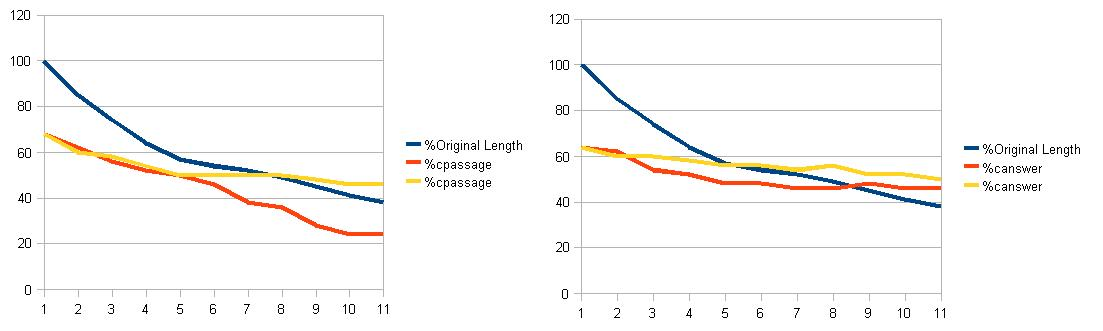
\includegraphics[scale = 0.50]{IS1008c_summaries.jpg}
\caption{Schemas for IS1008c summaries}
\label{schema: Results for IS1008c summaries}
\end{figure}

\begin{table}[htb!]
 \tiny
\caption{Results for IB4010 summaries}
\begin{tabular}{|c|c|c|c|c|c|}
\hline
\multicolumn{ 1}{|c|}{\%Original Length \tnote{*}} & \multicolumn{ 3}{c|}{ASR Summaries} & \multicolumn{ 2}{c|}{Random Summaries} \\ \cline{ 2- 6}
\multicolumn{ 1}{|c|}{} & rank score & \%cpassage & \%canswer & \%cpassage & \%canswer \\ \hline
100 & \ensuremath{\geq0.00} & 45 & 62 & 45 & 62 \\ \hline
85 & \ensuremath{\geq0.05} & 34 & 51 & 44 & 59 \\ \hline
74 & \ensuremath{\geq0.10} & 26 & 55 & 38 & 56 \\ \hline
65 & \ensuremath{\geq0.15} & 21 & 52 & 37 & 56 \\ \hline
58 & \ensuremath{\geq0.20} & 21 & 54 & 37 & 56 \\ \hline
54 & \ensuremath{\geq0.25} & 20 & 52 & 36 & 56 \\ \hline
51 & \ensuremath{\geq0.30} & 17 & 53 & 36 & 54 \\ \hline
47 & \ensuremath{\geq0.35} & 17 & 53 & 36 & 55 \\ \hline
44 & \ensuremath{\geq0.40} & 16 & 52 & 33 & 54 \\ \hline
40 & \ensuremath{\geq0.45} & 14 & 50 & 35 & 52 \\ \hline
36 & \ensuremath{\geq0.50} & 15 & 51 & 33 & 52 \\ \hline
\end{tabular}
\begin{tablenotes}
\item[*] Original length of ASR transcript for IB4010 is 4624 words 
\end{tablenotes}
\label{tab: Results for IB4010 summaries}
\end{table}


\begin{figure}[hb!]
\centering
 \scriptsize
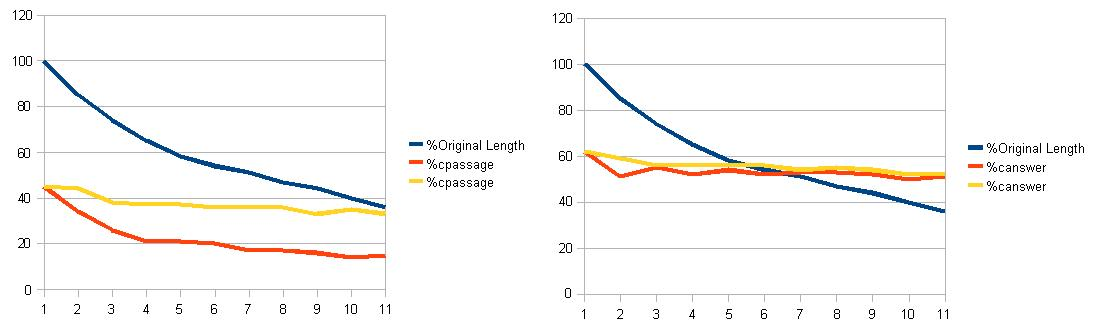
\includegraphics[scale = 0.50]{IB4010_summaries.jpg}
\caption{fig: Schemas for IB4010 summaries}
\label{schema: Schemas for IB4010 summaries}
\end{figure}

\normalsize

\pagebreak
\subsubsection*{Parameter Optimization}
The task of the parameter optimisation is to find parameters which are the best fit for each transcript IB4010 and IS1008c. These parameters are search window size and search window step. The goal is to use obtainned parameters for evaluation methods in the remains of this chapter.

For this, we use 5-fold Cross-Validation method as presented in the previous chapter to build a statistic table. This table consists of columns and rows which present values of window step and values of window size correspondingly, for instance, for position (2,5), the step of search window is 2 x input question size and the size is 5 x input question size. In which, each position (row,column) of the table present number of partitions as training data of Cross-Validation method that obtain maximal scores using the value of parameters corresponding to row and column of this position. For instance, the first partition obtains maximal scores at (2,3), (2,5) and the second partition obtain maximal score at (2,4), (2,5) and the others partitions obtain maximal scores at other pairs of parameters, then value of the position (2,5) of the table is 2 corresponding to two partitions. That means when search window size is 2 and search window is 5, there are two partitions over all five partitions obtain maximal score. The maximal scores are the maximal number of true passages retrieved by the algorithm in the first phase. For this experiment, we only use the first phase Passage Retrieval because it is the most essential of the proposed algorithm.

The following tables present results obtainned for IB4010 and IS1008c in detail:


 \scriptsize
\begin{center}
\begin{threeparttable}
\caption{Parameter Optimization for IB4010}
\begin{tabular}{|>{\bf}c|c|c|c|c|c|c|c|c|c|c|c|c|c|}
\hline \backslashbox{Size}{Step} & \bf{1} & \bf{2} & \bf{3} & \bf{4} & \bf{5} & \bf{6} & \bf{7} & \bf{8} & \bf{9} & \bf{10} & \bf{11} & \bf{12} & \bf{13} \\ 
\hline 1 &  &  &  &  &  &  &  &  &  &  &  &  &  \\ 
\hline 2 &  &  &  &  &  &  &  &  &  &  &  &  &  \\ 
\hline 3 &  &  &  &  &  &  &  &  &  &  &  &  &  \\ 
\hline 4 &  &  &  &  &  &  &  &  &  &  &  &  &  \\ 
\hline 5 &  &  &  &  &  &  &  &  &  &  &  &  &  \\ 
\hline 6 &  &  &  &  &  &  &  &  &  &  &  &  &  \\ 
\hline 7 &  &  &  &  &  &  &  &  &  &  &  &  &  \\ 
\hline 8 & 1 &  &  & 1 &  &  &  &  &  &  &  &  &  \\ 
\hline 9 & 4 & 3 &  &  &  &  &  &  &  &  &  &  &  \\ 
\hline 10 & 4 & 2 &	\multicolumn{1}{>{\columncolor{yellow}}c}{5}\tnote{*} &  &  &  &  &  &  &  &  &  &  \\ 
\hline 11 & 3 & 2 & 5 &  &  &  &  &  &  &  &  &  &  \\ 
\hline 12 & 1 &  &  &  &  &  &  &  &  &  &  &  &  \\ 
\hline 13 &  & 1 & 2 &  &  &  &  &  &  &  & 1 &  &  \\ 
\hline 
\end{tabular}
\begin{tablenotes}
\item[*] This position is chosen
\end{tablenotes}
\end{threeparttable}
\end{center}



\begin{center}
\begin{threeparttable}
\caption{Parameter Optimization for IS1008c}
%\begin{tabular}{|>{\bf}c|>{\sc}c|}
\begin{tabular}{|>{\bf}c|c|c|c|c|c|c|c|c|c|c|c|c|c|}
\hline \backslashbox{Size}{Step}  & \bf{1} & \bf{2} & \bf{3} & \bf{4} & \bf{5} & \bf{6} & \bf{7} & \bf{8} & \bf{9} & \bf{10} & \bf{11} & \bf{12} & \bf{13} \\ 
\hline 1 &  &  &  &  &  &  &  &  &  &  &  &  &  \\ 
\hline 2 & 1 &  &  &  &  &  &  &  &  &  &  &  &  \\ 
\hline 3 & 1 & 1 & 1 &  &  &  &  &  &  &  &  &  &  \\ 
\hline 4 & \multicolumn{1}{>{\columncolor{yellow}}c}{4}\tnote{*} & 1 & 1 & 1 &  &  &  &  &  &  &  &  &  \\ 
\hline 5 &  &  & 1 & 1 &  &  &  &  &  &  &  &  &  \\ 
\hline 6 & 2 & 2 & 3 & 1 & 2 & 1 &  &  &  &  &  &  &  \\ 
\hline 7 & 1 &  & 3 &  & 2 & 1 &  &  &  &  &  &  &  \\ 
\hline 8 &  &  &  &  &  &  &  & 2 &  &  &  &  &  \\ 
\hline 9 & 3 & 1 & 1 & 1 & 1 & 1 &  &  &  &  &  &  &  \\ 
\hline 10 & 2 &   &	1 & 1 & 1 & 1 &  &  &  & 1 &  &  &  \\ 
\hline 11 & 1 & 1 &   &  &   & 1 & 1 &  &  & 1 &  &  &  \\ 
\hline 12 & 5 & 3 & 3 &  & 2 & 4 & 3 &  &  & 1 & 1 &  &  \\ 
\hline 13 & 1 & 2 & 3 &  & 3 &   & 1 &  &  & 1 & 1 &  &  \\ 
\hline 
\end{tabular}
\begin{tablenotes}
\item[*] This position is chosen 
\end{tablenotes}
\end{threeparttable}
\end{center}

\normalsize 

According to the way of table construction above, parameters are considered good if they help as many training data as possible obtain the maximal scores. Therefore, we will choose parameters at a position whose value is the largest in the table as the relevant parameters. As seen in the table, for IB4010, there are two maximal values at (10,3) and (11,3) and for IS1008c, the value of position (12,1) is the largest. These values of parameters help all training data of Cross-Validation method obtain the best scores. However, it is evident that more size of a search window increases, the higher probability that a passage becomes correct is. When the size of search window is as equal as the size of the transcript, then it certainly contains the information of the question. So the returned passage is always true. In this task, we want to find parameters that help programme obtain the maximal number of correct passages but the objective of the passage retrieval is to reduce the search space. For this reason, we should choose the smallest size of search window that is suitable for most partitions. In the table of IS1008c, the position (4,1) seems acceptable that is suitable for 4 over 5 training data. That means the size of search window is 4 and the step of search window is 1 are the best fit for the BET questions and the transcript IS1008c. 
In the table of IB4010, the pair of parameters (10,3) has the best value, thus the size of search window is 10 and the step of search window is 3 are chosen as the best fit for the BET question and the transcript IB4010.

As mentioned in the beginning of the section, the chosen parameters are applied in the next sections.




\pagebreak

\subsubsection*{Comparison with BET scores by human subjects}
 The main goal of this comparison is to know whether automatic machine and human subjects have the same difficulties to answer the BET questions. By analysing the scores obtainned by the system and BET scores, we can also identify in which case this system is useful to help humans answer the BET questions. 

The BET scores used for this comparison are results from BET for the TQB interface \cite{popescubelis2007otm} that is known as a Transcript-based Query and Browsing Interface which was developed by Andrei Popescu-Belis. The TQB is considered as a meeting browser tool for searching and browsing multi-modal recordings of group meetings. And the BET method is used to evaluate the performance of this meeting browser over two meetings IB4010 and IS1008c.

According to the BET method, human subjects, that did not work with TQB before, were tested by answering the BET questions using TQB. They were 28 students at the University of Geneva, mainly form the School of Translation and Interpreting. Half of the subjects started with IB4010 and continued with IS1008c, and the other half did the reverse order, thus allowing for differentiated results depending on whether a meeting was seen first or second. That means when subjects worked on first meetings, they were trained with the TQB interface, so that they would answer BET questions better on second meeting. In fact, the average of precision is a bit higher for the second meeting. In this experiment, both BET scores as the first meeting and the second meeting are used to compare with results obtainned by the system. However, only 8 BET questions for each meeting are used for this comparison.  In which we are interested in only two information of BET scores, they are time average of answering and precision for each answer. 

In order to set up configuration of the system, defined parameters of search window are obtainned from previous section Parameter Optimisation. They are (search window size = 10 x question size, search window step = 3 x question size) for IB4010 and (search window size = 4 x question size, search window step = 1 x question size) for IS1008c.

The BET scores by human subjects and scores obtainned by the system are showed in detail in two tables \ref{table: BET scores for IB4010} and \ref{table: BET scores for IS1008c}. In each table, for the scores by human subjects, \textit{Precis1} and \textit{avg time1} in millisecond are average precision and average time as the first meeting, \textit{Precis2} and \textit{avg time2} are average precision and average time in millisecond as the second meeting. For scores obtainned by the system, \textit{\#cpassage} and \textit{\#canswer} are number of correct passages and number of correct true-false answers correspondingly. However, number of answers for each question is only one. \textit{time} in millisecond is time for answering one question.




\begin{table}[htb!]
\scriptsize
\caption{Comparison with BET scores by human subjects for IB4010}
\begin{tabular}{|c|r|r|r|r|r|r|r|}
\hline
\multicolumn{ 1}{|c|}{curQuid} & \multicolumn{ 4}{c|}{Humans} & \multicolumn{ 3}{c|}{System} \\ \cline{ 2- 8}
\multicolumn{ 1}{|l|}{} & \multicolumn{1}{c|}{Precis1} & \multicolumn{1}{c|}{avg time1} & \multicolumn{1}{c|}{Precis2} & \multicolumn{1}{c|}{avg time2} & \multicolumn{1}{c|}{\#cpassage} & \multicolumn{1}{c|}{\#canswer} & \multicolumn{1}{c|}{\#time } \\ \hline
1 & 0.93 & 303.14 & 0.71 & 143 & 0 & 0 & 24 \\ \hline
2 & 0.93 & 105.36 & 1.00 & 66.14 & 1 & 1 & 22 \\ \hline
3 & 0.71 & 118.14 & 1.00 & 89.21 & 1 & 1 & 40 \\ \hline
4 & 0.86 & 207.5 & 0.86 & 206.43 & 1 & 1 & 32 \\ \hline
5 & 1.00 & 64.71 & 0.93 & 37 & 0 & 1 & 16 \\ \hline
6 & 0.93 & 57.79 & 1.00 & 53.21 & 1 & 1 & 17 \\ \hline
7 & 0.93 & 60.93 & 0.71 & 52 & 1 & 1 & 24 \\ \hline
8 & 0.71 & 129.5 & 0.79 & 85.29 & 1 & 1 & 19 \\ \hline
\multicolumn{1}{|l|}{} & \textbf{0.88} & \textbf{130.88} & \textbf{0.88} & \textbf{91.54} & \textbf{0.75} & \textbf{0.88} & \textbf{24.25} \\ \hline
\end{tabular}
\label{table: BET scores for IB4010}
\end{table}

%\begin{figure}[htb!]
%\scriptsize
%\centering
%\begin{minipage}{5cm}
%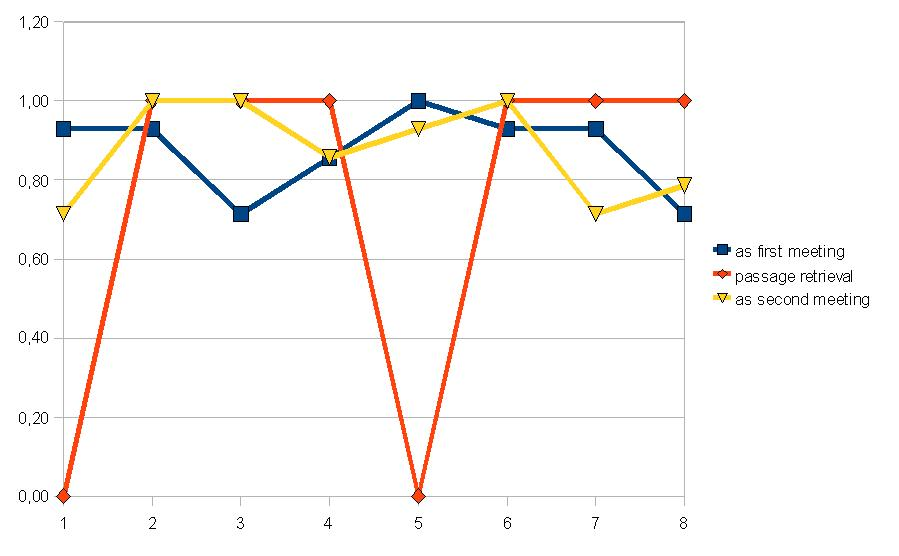
\includegraphics[width=1\textwidth]{BET_results_compararison_IB4010_passage.jpg}
%%\caption{Compararison with BET results for IS1008c (Passage retrieval)}
%\end{minipage}
%\hfill
%\begin{minipage}{5cm}
%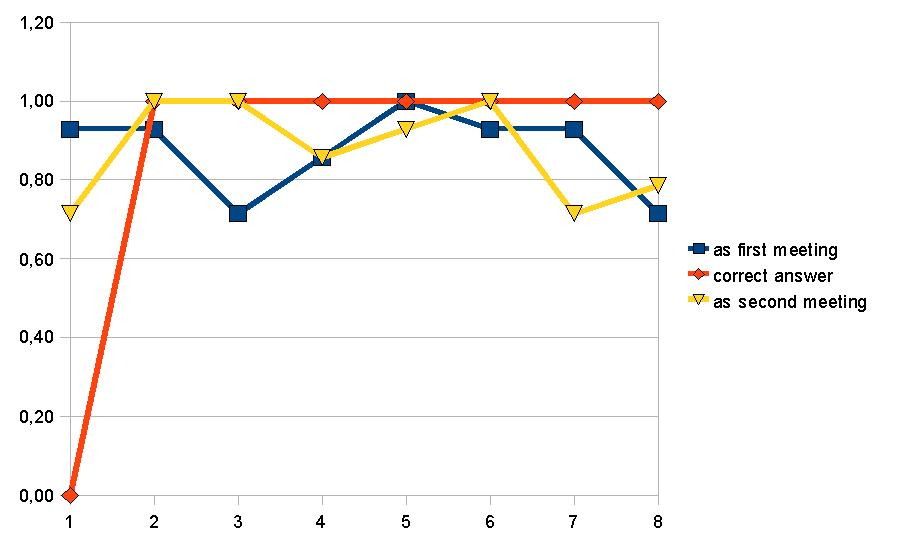
\includegraphics[width=1\textwidth]{BET_results_compararison_IB4010_truefalse.jpg}
%%\caption{Compararison with BET results for IS1008c (True-false questions answering}
%\end{minipage}
%\caption{Comparison with BET results for IB4010}
%\end{figure}
 




%Say that they come from previous study + reference

%Chu thich nguon du lieu tu BET, quota the paper on BET4TQB

According to the BET for TQB \cite{popescubelis2007otm}, average precision to answer all BET questions for IB4010 is 0.85 \ensuremath{\pm} 0.05 and 0.70 \ensuremath{\pm} 0.10 for IS1008c. Thus, for human subjects, we can divide the BET questions into two groups: easy and less easy. A BET question belongs to easy group as the first group if average precision of its answers as first meeting or second meeting is more than 0.85 for IB4010 and 0.70 for IS1008c, otherwise it belongs to the second group. Meanwhile, for the system, easy group includes all questions that  their number of correct passage or number of correct true-false answer is 1.
This help us have a standard to compare the BET scores by humans with scores obtainned by the system.

We examine first the results for IB4010. According to the convention above, for human subjects there is only one less easy question that is question numbered 8, meanwhile there are two less easy questions for the system which are questions number 1 and 5. In fact, all of these questions are deductive questions that require rather a comprehension deeply than a search of lexical similarities. In detail, the question numbered 1 is "throughout". That means it is necessary to read all transcript before answering the question. That is why the system could not identify the correct passage using a small search window that does not cover all information of the transcript as it requires for this type of question. Consequently, the true-false answer is determined by chance that is false in this case. The question numbered 5 also require a deduction for its true statement "No one had seen Goodfellas". In the meeting, when all meeting participants said "No" for question "Have you seen Goodfellas?", it is easy for human subjects to understand the answer of participants. However, this is really a difficult task for an automatic system.  Therefore, the system identified incorrect passage. Consequently, its true-false answer is determined by chance, that is true in this case. The question numbered 8 is also a deductive question because it is not easy to match the question "I dislike Quentin" with the text "I am not a huge fan of Quentin". However, the system gave true answer for this question meanwhile it made difficult to human subjects. That is because the keyword Quentin appears only one time in the transcript and the system based on this word but did not based on the meaning of the essential phrase to identify correct passage.

\begin{table}[ht!]
\scriptsize
\caption{Comparison with BET scores by human subjects for IS1008c}
\begin{tabular}{|c|r|r|r|r|r|r|r|}
\hline
\multicolumn{ 1}{|c|}{curQuid} & \multicolumn{ 4}{c|}{Humans} & \multicolumn{ 3}{c|}{System} \\ \cline{ 2- 8}
\multicolumn{ 1}{|l|}{} & \multicolumn{1}{c|}{Precis1} & \multicolumn{1}{c|}{avg time1} & \multicolumn{1}{c|}{Precis2} & \multicolumn{1}{c|}{avg time2} & \multicolumn{1}{c|}{\#cpassage} & \multicolumn{1}{c|}{\#canswer} & \multicolumn{1}{c|}{\#time} \\ \hline
1 & 0.86 & 410 & 0.93 & 127.36 & 1 & 1 & 13 \\ \hline
2 & 0.67 & 298.58 & 0.86 & 129.5 & 1 & 1 & 45 \\ \hline
3 & 0.82 & 78.09 & 0.93 & 67.5 & 1 & 1 & 15 \\ \hline
4 & 0.89 & 80.22 & 0.93 & 103.93 & 1 & 1 & 16 \\ \hline
5 & 0.63 & 66.38 & 0.69 & 63.92 & 1 & 0 & 20 \\ \hline
6 & 0.67 & 44 & 0.73 & 62.18 & 0 & 0 & 10 \\ \hline
7 & 1.00 & 24 & 0.82 & 48 & 1 & 0 & 11 \\ \hline
8 & 0.67 & 66 & 0.64 & 93.55 & 0 & 1 & 11 \\ \hline
\multicolumn{1}{|l|}{} & \textbf{0.77} & \textbf{133.41} & \textbf{0.81} & \textbf{86.99} & \textbf{0.75} & \textbf{0.63} & \textbf{17.63} \\ \hline
\end{tabular}
\label{table: BET scores for IS1008c}
\end{table}

For IS1008c, as defined above for easy and less easy questions, there are two less easy questions for human subjects. They are questions numbered 5 and 8. For the system, it answered wrong three questions that are questions numbered 5, 6,7 and 8. In which, the questions numbered 5, 6 and 8 are deductive questions. For question numbered 5, whose true statement is "Agnes express her opinion that ...", the correct passage should be "Agnes: I think ... ". Two different expressions make difficult to understand for both human subjects and the automatic system. Dealing with the question numbered 6, which is "Agnes notes some reasons to not have a display", Agnes showed a list of reasons in the transcript but there is few matched words between question string and answer string. This is similar with the question numbered 8. However, the true-false answer for question numbered 8 is correct by chance. The question numbered 7 is not difficult so that the system gave correct passage but incorrect true-false answer. That means true-false answers by the system are not as stable as correct passage answering




In conclusion, although both human subjects and the system meet difficulties to answer deductive questions but it seems be more difficult for the automatic system. For IB4010, there are 3 deductive questions and the automatic system wrong answers 2 over 3 questions, meanwhile the human subjects have only difficulties to answer 1 over 3 questions. For IS1008c, there are also 3 deductive questions. The system gave wrong answers for all three questions, meanwhile the human subjects have difficulties to answer two questions. In fact, deductive questions are equivalent to How and Why questions that are difficult for all question answering systems \cite{prager2000qap, brill2002diq}.
According to experimental results, the results for passage retrieval are more logical than the results for true-false answers. That means the system should be developed to help humans answer BET-typed questions by identifying relevant passage instead of giving final answers.  In other words, it is a useful tool for locating answer, not necessarily finding it.






%\begin{figure}[htb!]
%\centering
%\begin{minipage}{5cm}
%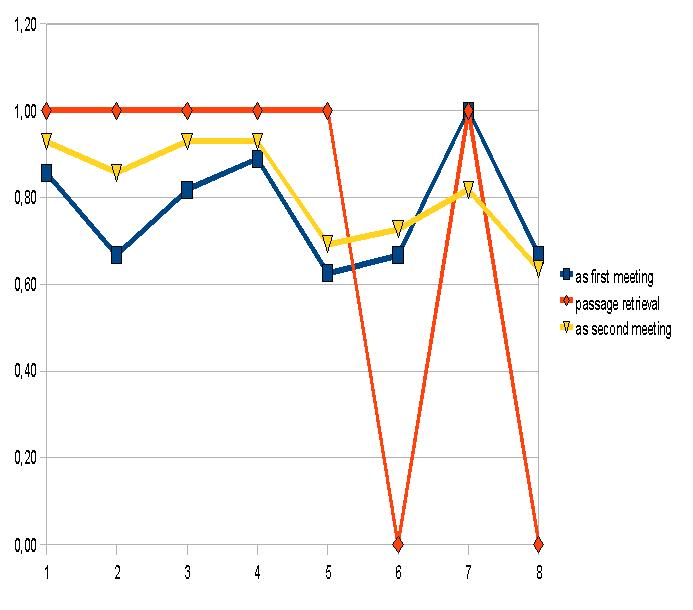
\includegraphics[width=1\textwidth]{BET_results_compararison_IS1008c_passage.jpg}
%%\caption{Compararison with BET results for IS1008c (Passage retrieval)}
%\end{minipage}
%\hfill
%\begin{minipage}{5cm}
%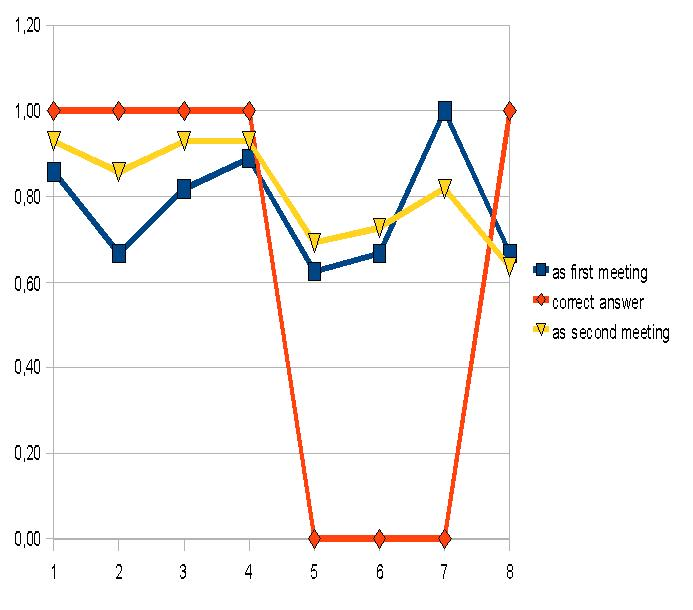
\includegraphics[width=1\textwidth]{BET_results_compararison_IS1008c_truefalse.jpg}
%%\caption{Compararison with BET results for IS1008c (True-false questions answering}
%\end{minipage}
%\caption{Comparison with BET results for IS1008c}
%\end{figure}

% + add last paragraph from page 29 here.
% 5.4 = very good comparison, exactly what I expected from you! Only needs some better explanatation.


\pagebreak
\label{Bibliography}
\bibliographystyle{plain}
\bibliography{biblio} 

\end{document}